\documentclass[SingleSpace,12pt,Journal]{Serre_ASCE}
\usepackage[dvips]{graphicx}
\usepackage[dvipsnames]{xcolor}
\usepackage{amsmath}
\usepackage{amsfonts}
\usepackage{amssymb}
\usepackage{lineno}
\usepackage{enumerate}
\usepackage{url}
\usepackage{times}
\usepackage{subfigure}
\usepackage[skip=0pt]{caption}

% TIME ON EVERY PAGE AS WELL AS THE FILE NAME
\usepackage{fancyhdr}
\usepackage{currfile}
\usepackage[us,12hr]{datetime} % `us' makes \today behave as usual in TeX/LaTeX
\fancypagestyle{plain}{
\fancyhf{}
\rfoot{\small Draft Paper \\ File Name: {\currfilename} \\ Date: {\ddmmyyyydate\today} at \currenttime}
\lfoot{Page \thepage}
\renewcommand{\headrulewidth}{0pt}}
\pagestyle{plain}

\newcommand\solidrule[1][0.25cm]{\rule[0.5ex]{#1}{1pt}}
\newcommand\dashedrule{\mbox{%
  \solidrule[2mm]\hspace{2mm}\solidrule[2mm]}}
 
\newcommand{\dotrule}[1]{%
   \parbox{#1}{\dotfill}} 

\begin{document}

\title{Behaviour of the Dam-Break Problem for the Serre Equations}

\author{
Jordan~Pitt,%
\thanks{Mathematical Sciences Institute, Australian National University, Canberra, ACT 0200, Australia, E-mail: Jordan.Pitt@anu.edu.au. The work undertaken by the first author was supported financially by an Australian National University Scholarship.}
\\
Christopher~Zoppou,\footnotemark[1]%
%
% Adding a second author with the same affiliation (still using \thanks):
\\
Stephen~G.~Roberts,\footnotemark[1]
}

\maketitle

\begin{abstract}

\end{abstract}

\KeyWords{dispersive waves, conservation laws, Serre equation, finite volume method, finite difference method}

\linenumbers

%--------------------------------------------------------------------------------
\section{Introduction} \label{intro} 

%--------------------------------------------------------------------------------
\section{Serre Equations}
\label{section:Serre Equations}
The Serre equations can derived as an approximation to the full Euler equations by depth integration similar to \cite{Su-Gardener-1969-536}. They can also be seen as an asymptotic expansion of the Euler equations \cite{Bonneton-Lannes-2009-16601}. The former is more consistent with the perspective from which numerical methods will be developed while the latter indicates the appropriate regions in which to use these equations as a model for fluid flow.
\begin{figure}[htb]
\begin{center}
\includegraphics[width=7.0cm]{pics/explainers/one-dimensional-axis_Serre.eps}
\end{center}
\caption{The notation used for one-dimensional flow governed by the Serre equation.}
\label{fig:Notation}
\end{figure}
The scenario under which the Serre approximation is made consists of a two dimensional $\textbf{x} = (x,z)$ fluid over a bottom topography as in Figure \ref{fig:Notation} acting under gravity. Consider a fluid particle at depth  $\xi(\textbf{x},t) = h(x,t) + z_b(x) - z$ below the water surface, see Figure \ref{fig:Notation}. Where the water depth is $h(x,t)$ and $z_b(x)$ is the bed elevation. The fluid particle is subject to the pressure, $p(\textbf{x},t)$ and  gravitational acceleration, $\textbf{g} = (0,g)^T$ and has a velocity $\textbf{u} = (u(\textbf{x},t),w(\textbf{x},t))$,  where $u(\textbf{x},t)$ is the velocity in the $x$-coordinate and $w(\textbf{x},t)$ is the velocity in the $z$-coordinate and $t$ is time. Assuming that $z_b(x)$ is constant the Serre equations read \cite{Guyenne-etal-2014-169}
\begin{linenomath*}
\begin{subequations}\label{eq:Serre_nonconservative_form}
\begin{gather}
\dfrac{\partial h}{\partial t} + \dfrac{\partial (\bar{u}h)}{\partial x} = 0
\label{eq:Serre_continuity}
\end{gather}
\begin{gather}
\underbrace{\underbrace{\dfrac{\partial (\bar{u}h)}{\partial t} + \dfrac{\partial}{\partial x} \left ( \bar{u}^2h + \dfrac{gh^2}{2}\right )}_{\text{Shallow Water Wave Equations}} + \underbrace{\dfrac{\partial}{\partial x} \left (  \dfrac{h^3}{3} \left [ \dfrac{\partial \bar{u} }{\partial x} \dfrac{\partial \bar{u}}{\partial x} - \bar{u} \dfrac{\partial^2 \bar{u}}{\partial x^2}  - \dfrac{\partial^2 \bar{u}}{\partial x \partial t}\right ] \right )}_{\text{Dispersion Terms}} = 0.}_{\text{Serre Equations}}
\label{eq:Serre_momentum}
\end{gather}
\end{subequations}
\end{linenomath*}
Where $\bar{u}$ is the average of $u$ over the depth of water. 
\subsection{Conservation of mass and momentum}
The Serre equations are based on conservation of mass and momentum, thus our numerical methods should reflect this property. The total of a quantity $q$ in a system is measured by

\begin{gather}
\label{eqn:Condef}
\mathcal{C}_q(t) = \int_{-\infty}^{\infty} q\, dx
\end{gather}
so that we have for all $t$ both $\mathcal{C}_{h}(0) = \mathcal{C}_{h}(t)$ and $\mathcal{C}_{\bar{u}h}(0) = \mathcal{C}_{\bar{u}h}(t)$ representing conservation of mass and momentum respectively.

\subsection{Hamiltonian}

The Serre equations admit a Hamiltonian \cite{Li-Y-2002,Hank-etal-2010-2034,Green-Naghdi-1976-237}

\begin{gather}
\label{eqn:Hamildef}
\mathcal{H}(t) = \frac{1}{2}\int_{-\infty}^{\infty} hu^2 + gh^2 + \frac{h^3}{3} \left(\frac{\partial u}{\partial x}\right)^2\, dx
\end{gather}
where the bar over $u$ has been dropped to simplify notation. The Hamiltonian is such that $\mathcal{H}(t) = \mathcal{H}(0)$ for all times $t$.

We can calculate this numerically by partitioning the total integral into cell-wise integrals. The cell-wise integral can then be calculated by quartic interpolation utilising neighbouring cells and then applying Gaussian quadrature with $3$ points over the cell to get a sufficiently high order method to calculate the Hamiltonian, in particular this method is at least third order accurate for the $\partial u / \partial x$ term. 
%--------------------------------------------------------------------------------
\section{Direct Numerical Methods} 
\label{sec:DirNumMet}
%--------------------------------------------------------------------------------
The presence of the mixed spatial temporal derivatives in the momentum equation \eqref{eq:Serre_momentum} makes the Serre equations difficult to solve with standard numerical methods. A naive way to avoid this is to approximate \eqref{eq:Serre_momentum} by finite differences and the results of this are presented here. To facilitate this a uniform grid in space will be used with $\Delta x  = x_{i+1} - x_i$ for all $i$. Quantities evaluated at these grid points will be denoted by subscripts for example $h_i = h(x_i)$. The grid in time is also uniform and will be denoted by superscripts for example $h^n = h(t^n)$, note that $h^n$ is a function in space. 
\subsection{Finite Difference Appximation to Conservation of Momentum Equation} 
\label{subsec:FDA2conmom}
In [][Zoppou thesis/my work] it was demonstrated that an efficient numerical scheme for the Serre equations must be at least second-order accurate thus the derivatives in \eqref{eq:Serre_momentum} will be approximated by second-order finite differences. Firstly \eqref{eq:Serre_momentum} must be expanded, making use of \eqref{eq:Serre_continuity} one obtains
\begin{linenomath*}
\begin{subequations}
\begin{gather}
h\dfrac{\partial u}{\partial t} + X - h^2\frac{\partial^2 u}{\partial x \partial t} - \frac{h^3}{3}\frac{\partial^3 u}{\partial x^2 \partial t}  =0 
\label{eq:expandedu}
\end{gather}
where $X$ contains only spatial derivatives and is
\begin{gather}
X = uh\frac{\partial u}{\partial x} + gh\frac{\partial h}{\partial x} + h^2\frac{\partial u}{\partial x}\frac{\partial u}{\partial x} + \frac{h^3}{3}\frac{\partial u}{\partial x}\frac{\partial^2 u}{\partial x^2} - h^2u\frac{\partial^2 u}{\partial x^2}- \frac{h^3}{3}u\frac{\partial^3 u}{\partial x^3} .
\end{gather}
\end{subequations}
\end{linenomath*} Taking the second-order centred finite difference approximation to the spatial and temporal derivatives for \eqref{eq:expandedu} after some rearranging gives
\begin{linenomath*}
\begin{gather}
h^{n}_iu^{n+1}_i - \left(h^{n}_i\right)^2 \left(\frac{u^{n+1}_{i+1} -u^{n+1}_{i-1} }{2 \Delta x}\right) - \frac{\left(h^{n}_i\right)^3}{3}\left(\frac{u^{n+1}_{i+1} - 2u^{n+1}_{i} + u^{n+1}_{i-1} }{\Delta x^2}\right) = - Y^n_i 
\label{eq:expandedutdisc3}
\end{gather}
\end{linenomath*}
where
\begin{linenomath*}
\begin{gather*}
Y_i^n = 2\Delta tX_i^{n} - h_i^{n}u_i^{n-1} + \left(h_i^{n}\right)^2\left(\frac{u^{n-1}_{i+1} -u^{n-1}_{i-1} }{2 \Delta x}\right) + \frac{\left(h_i^{n}\right)^3}{3}\left(\frac{u^{n-1}_{i+1} - 2u^{n-1}_{i} + u^{n-1}_{i-1} }{\Delta x^2}\right) .
\label{eq:expandfactor Xp}
\end{gather*}
\end{linenomath*}
Equation \eqref{eq:expandedutdisc3} can be rearranged into a tri-diagonal matrix that updates $u$ given its current and previous values. So that
\begin{linenomath*}
\begin{gather}
\left[\begin{array}{c}
 u^{n+1}_0 \\
 \vdots \\
 u^{n+1}_m \end{array}\right]
 = A^{-1} \left[\begin{array}{c}
  -Y^n_0 \\
  \vdots \\
  -Y^n_m \end{array}\right] =: \mathcal{G}_u\left(\boldsymbol{u}^n,\boldsymbol{h}^n, \boldsymbol{u}^{n-1},\boldsymbol{h}^{n-1}, \Delta x, \Delta t \right).
\label{eq:FDcentforu}
\end{gather}
\end{linenomath*}
In particular this is an explicit [?] numerical method for \eqref{eq:Serre_momentum}, that requires the current and previous values of $h$ and $u$.


\subsection{The Lax Wendroff Method for Conservation of Mass Equation}
\label{section:}
Because the conservation of mass equation \eqref{eq:Serre_continuity} has no mixed derivative term standard numerical techniques for conservation laws can be used. In particular the Lax-Wendroff method can be used as done by \citeN{El-etal-2006}, here we present the method in replicable detail.

Note that \eqref{eq:Serre_continuity} is in conservative law form for $h$ where the flux is $uh$. Thus using the previously defined spatio-temporal discretisation the two step Lax-Wendroff update[] for $h$ is
\begin{linenomath*}
\begin{gather}
h^{n + 1/2}_{i+ 1/2} = \frac{1}{2}\left(h^{n}_{i+1} + h^{n}_i\right) - \frac{\Delta t}{2\Delta x}\left(u^n_{i+1}h^n_{i+1} - h^n_{i}u^n_{i}\right),
\end{gather}
\begin{gather}
h^{n + 1/2}_{i- 1/2} = \frac{1}{2}\left(h^{n}_{i} + h^{n}_{i-1}\right) - \frac{\Delta t}{2\Delta x}\left(u^n_{i}h^n_{i} - h^n_{i-1}u^n_{i-1}\right),
\end{gather}
\begin{gather}
h^{n+1}_i = h^{n}_i - \frac{\Delta t}{\Delta x}\left(u^{n + 1/2}_{i+ 1/2}h^{n + 1/2}_{i+ 1/2} - u^{n + 1/2}_{i- 1/2}h^{n + 1/2}_{i- 1/2}\right).
\label{eq:LW4h}
\end{gather}
\end{linenomath*}
To calculate $u^{n + 1/2}_{i \pm 1/2}$ first $u$ is advanced in time by $\mathcal{G}_u$ then using linear interpolation in both space and time gives
\begin{gather}
u^{n + 1/2}_{i+ 1/2} = \frac{u^{n+1}_{i+1} + u^{n}_{i+1} + u^{n+1}_{i} + u^{n}_{i} }{4},
\end{gather}
\begin{gather}
u^{n + 1/2}_{i- 1/2} = \frac{u^{n}_{i} + u^{n}_{i} + u^{n+1}_{i-1}+ u^{n}_{i-1} }{4}.
\end{gather}
Thus we have the following update scheme
\begin{linenomath*}
\begin{gather}
\left[ \begin{array}{l}
\boldsymbol{h}^{n+1} \\
\boldsymbol{u}^{n+1}
 \end{array}\right] = \mathcal{E}\left(\boldsymbol{u}^n,\boldsymbol{h}^n, \boldsymbol{u}^{n-1},\boldsymbol{h}^{n-1}, \Delta x, \Delta t \right). 
\end{gather}
\end{linenomath*}

%--------------------------------------------------------------------------------
\subsection{Second Order Naive Finite Difference Method}
%--------------------------------------------------------------------------------
Here we also present a completely naive method for comparative purposes, to do this we apply the procedure used above on \eqref{eq:Serre_momentum} to \eqref{eq:Serre_continuity}. Thus the derivatives were first expanded then approximated by second order centered finite differences after rearranging this to give an update formula we obtain
\begin{linenomath*}
\begin{gather}
h^{n+1}_i = h^{n-1}_i - \Delta t \left(u^{n}_{i}\frac{h^{n}_{i+1} - h^{n}_{i-1}}{\Delta x} + h^{n}_{i}\frac{u^{n}_{i+1} - u^{n}_{i-1}}{\Delta x}\right).
\end{gather}
\end{linenomath*}
Preforming this update for all $i$ will be denoted by $\mathcal{G}_h\left(\boldsymbol{u}^n,\boldsymbol{h}^n,\boldsymbol{h}^{n-1} ,\Delta x, \Delta t \right)$.
Thus we get the naive second-order centred finite difference method for the Serre equations
\begin{linenomath*}
\begin{gather}
\left.
\begin{array}{l l}
\boldsymbol{h}^{n+1}&=\mathcal{G}_h\left(\boldsymbol{u}^n,\boldsymbol{h}^n, \Delta x, \Delta t \right) \\
\boldsymbol{u}^{n+1}&=\mathcal{G}_u\left(\boldsymbol{u}^n,\boldsymbol{h}^n, \boldsymbol{u}^{n-1},\boldsymbol{h}^{n-1}, \Delta x, \Delta t \right)
\end{array} \right\rbrace \mathcal{G}\left(\boldsymbol{u}^n,\boldsymbol{h}^n, \boldsymbol{u}^{n-1},\boldsymbol{h}^{n-1}, \Delta x, \Delta t \right).
\end{gather}
\end{linenomath*}
%-------------------------------------------------------------------------------- 
\section{Conservative Form of The Serre Equations}
To overcome the aforementioned difficulty of mixed derivatives the Serre equations \eqref{eq:Serre_nonconservative_form} can be reformulated into conservative form. This is accomplished by the introduction of a new quantity \cite{Hank-etal-2010-2034,Zoppou-2014}
\begin{linenomath*}
\begin{gather}
\label{eq:Gdefinition}
G = uh - h^2 \dfrac{\partial h}{\partial x} \dfrac{\partial u}{\partial x} - \frac{h^3}{3} \dfrac{\partial^2 u}{\partial x^2}.
\end{gather}
\end{linenomath*}
Consequently, \eqref{eq:Serre_nonconservative_form} can be rewritten as
\begin{linenomath*}
\begin{subequations}
\begin{gather}
\dfrac{\partial h}{\partial t} + \dfrac{\partial (uh)}{\partial x} = 0
\label{eq:Serrecon_continuity}
\end{gather}
and
\begin{gather}
\dfrac{\partial G}{\partial t} + \dfrac{\partial}{\partial x}\left(Gu + \dfrac{gh^2}{2} - \dfrac{2h^3}{3}\dfrac{\partial u}{\partial x}\dfrac{\partial u}{\partial x}\right) = 0.
\label{eq:Serrecon_momentum}
\end{gather}
\label{eq:Serrecon}
\end{subequations}
\end{linenomath*}

\subsection{A Hybrid Finite Difference-Volume Method for Serre Equations in Conservative Form}
\label{section:hybridmethod}
%--------------------------------------------------------------------------------
The conservative form \eqref{eq:Serrecon} allows for a wider range of numerical techniques such as finite element methods \cite{Guyenne-etal-2014-169} and finite volume methods \cite{Hank-etal-2010-2034,Zoppou-2014}. In this paper the first ($\mathcal{V}_1$), second ($\mathcal{V}_2$) and third-order ($\mathcal{V}_3$) finite difference-volume methods (FDVM) of [] will be used. These have been validated and their order of accuracy confirmed.

\subsection{Stability Condition} 
To ensure stability of the FDVMs the time-step $\Delta t$ must satisfy the Courant-Friedrichs-Lewy (CFL) criteria \cite{Harten-etal-1983-357}

\begin{gather}
\label{eq:CFL}
\Delta t < \frac{Cr \Delta x}{2\max \left\lbrace |\lambda| \right\rbrace}
\end{gather}

 with $0<Cr\le 1$ where $\lambda$ is the wave speed. For the Serre equations it has been demonstrated that the wave speed is bounded by the wave speed of the Shallow Water Wave equations.[zoppou]

\section{Numerical Simulations}
\label{section:Numerical Simulations}
%--------------------------------------------------------------------------------
In this section the methods introduced in this paper will be validated by using them to approximate an analytic solution of the Serre equations, this will also be used to verify their order of accuracy. Then an in depth comparison of these methods for a smooth approximation to the discontinuous dam break problem will be provided to investigate the behaviour of these equations in the presence of discontinuities. This is a problem that so far has only received a proper treatment in \cite{El-etal-2006}, with other research giving only a cursory investigation into the topic. 

%--------------------------------------------------------------------------------
\section{Soliton}
\label{section:Convergence Rate}
%--------------------------------------------------------------------------------
Currently cnoidal waves are the only family of analytic solutions to the Serre equations \cite{Carter-Cienfuegos-2010-259}. Solitons are a particular instance of cnoidal waves that travel without deformation and have been used to verify the convergence rates of the described methods in this paper. 

For the Serre equations the solitons have the following form
\begin{linenomath*}
\begin{subequations}
\begin{gather}
h\left(x,t\right) = a_0 + a_1\text{sech}^2\left( \kappa\left(x - ct\right)\right),
\end{gather}
\begin{gather}
u\left(x,t\right) = c\left(1 - \dfrac{a_0}{h(x,t)} \right),
\end{gather}
\begin{gather}
\kappa = \dfrac{\sqrt{3a_1}}{2a_0 \sqrt{ a_0 + a_1}}
\end{gather}
and
\begin{gather}
c = \sqrt{g \left(a_0 + a_1\right)}
\end{gather}
\end{subequations}
\label{eq:sol}
\end{linenomath*}
where $a_0$ and $a_1$ are input parameters that determine the depth of the quiescent water and the maximum height of the soliton above that respectively. In the simulation $a_0 = 1\text{m}$, $a_1 = 1\text{m}$ for $x\in\left[-50\text{m},250\text{m}\right]$ and $t\in\left[0\text{s},50\text{s}\right]$. With $\Delta t = 0.5 \lambda^{-1} \Delta x$ where $\lambda = \sqrt{g \left(a_0 + a_1\right)}$ which is the maximum wave speed, this satisfies the CFL condition \eqref{eq:CFL}. 

%--------------------------------------------------------------------------------
\subsection{Results}
%--------------------------------------------------------------------------------
This numerical experiment and its results for the FDVM have been reported by [], this paper only reports the results for $\mathcal{G}$ and $\mathcal{E}$. 

From Figure \ref{fig:FDsolh} it can be seen that $\mathcal{G}$ and $\mathcal{E}$ accurately model the highly non-linear soliton problem reproducing the analytic solution up to graphical accuracy with the same $\Delta t$ and $\Delta x$ as in []. This demonstrates that for smooth problems both the FD and FDVM are comparable when using similar spatial and temporal resolutions. 

To demonstrate that in fact $\mathcal{E}$ and $\mathcal{G}$ are consistent, three measures were used. The first measures the relative distance of the numerical results for $h$ and $u$ from the analytic solution, it is defined for a general quantity $q$ and an approximation to it $q^*$ at $n$ values

\begin{gather}
L_1 = \dfrac{\sum_{i = 0}^{n} \left| q_i - q^*_i\right|}{\sum_{i = 0}^{n} \left| q_i\right|}.
\end{gather}
The second measures how well the schemes conserve a quantity $q$
\begin{gather}
C_1 = \dfrac{\left| \mathcal{C}_q(0) - \mathcal{C}_{q^*}(t_f) \right|}{\left| \mathcal{C}_q(0) \right|}
\end{gather}
where $t_f$ is the final time of the numerical experiment. For $\mathcal{C}_q(0)$ the analytic value is used while a numerical calculation is used for $\mathcal{C}_{q^*}(t_f)$ which for second-order methods is equivalent to taking the sum of all the $q^*_i$'s and then multiplying by $\Delta x$. For the Serre equations the conserved quantities are mass ($h$) and momentum ($uh$). Lastly how well the scheme conserves the Hamiltonian of the Serre equations is measured by 
\begin{gather}
H_1 = \dfrac{\left| \mathcal{H}(0) - \mathcal{H}(t_f) \right|}{\left| \mathcal{H}(0) \right|}
\end{gather}
where $t_f$ is the final time of the numerical experiment. For $\mathcal{H}(0)$ the analytic value is used while a numerical calculation is used for $\mathcal{H}(t_f)$.
%
\begin{figure}
\centering
\subfigure[][]{\label{fig:FDsolh}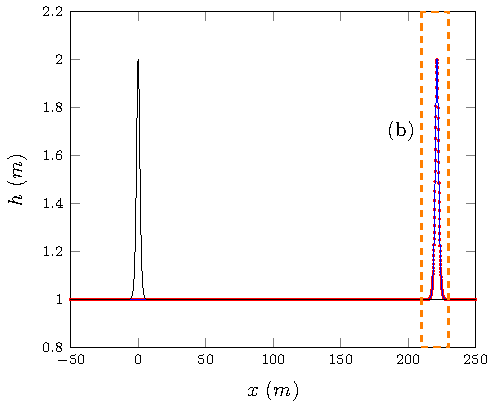
\includegraphics[width=7cm]{pics/results/soliton/ex/FDc.pdf}}
\subfigure[][]{\label{fig:FDsolhz} 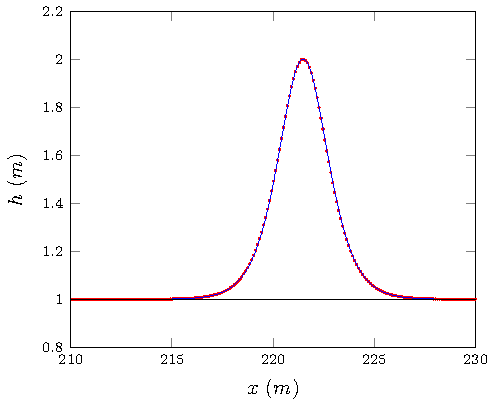
\includegraphics[width=7cm]{pics/results/soliton/ex/FDcz.pdf}}
\subfigure[][]{\label{fig:GRsolh}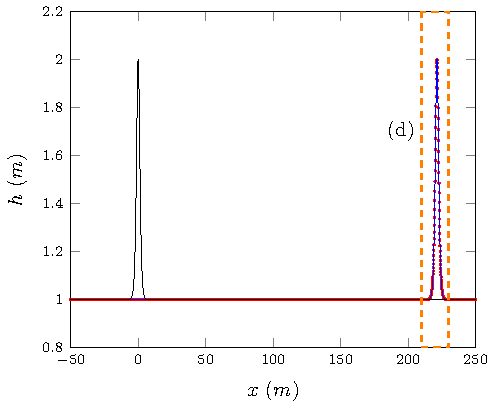
\includegraphics[width=7cm]{pics/results/soliton/ex/grim.pdf}}
\subfigure[][]{\label{fig:GRsolhz}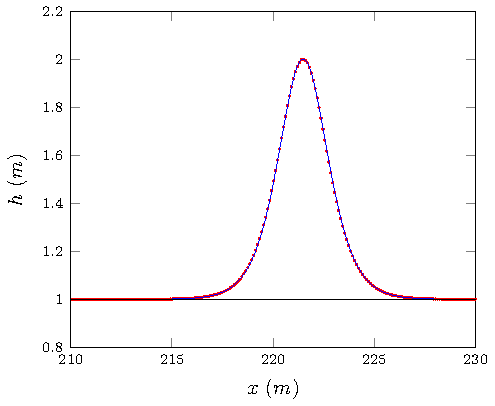
\includegraphics[width=7cm]{pics/results/soliton/ex/grimz.pdf}}
\caption{Water profile for the soliton problem \eqref{eq:sol} for $\mathcal{G}$ ((a),(b)) and $\mathcal{E}$ ((c),(d)) when $\Delta x = 10/2^{12}$ with the initial conditions ({\color{black} \solidrule}), analytic solution ({\color{blue} \solidrule}) and numerical result ({\color{red} $\bullet$}).}
\label{fig:FDMsolexp}
\end{figure}
\begin{figure}
\centering
\subfigure[][]{\label{fig:FDo2normL1}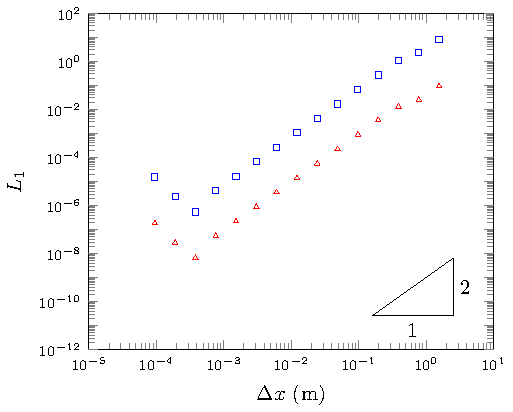
\includegraphics[width=7cm]{pics/results/soliton/L1/FDc.pdf}}
\subfigure[][]{\label{fig:FDo2Enorm}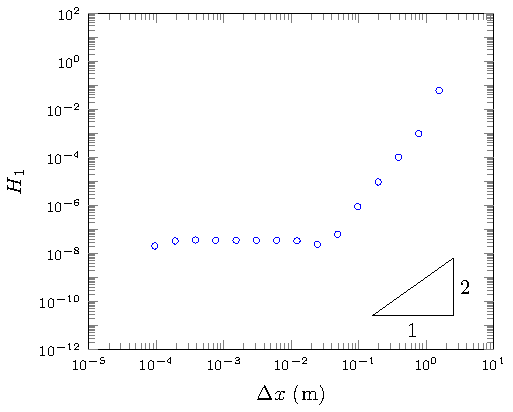
\includegraphics[width=7cm]{pics/results/soliton/H1/FDc.pdf}}
\subfigure[][]{\label{fig:grimo2normL1}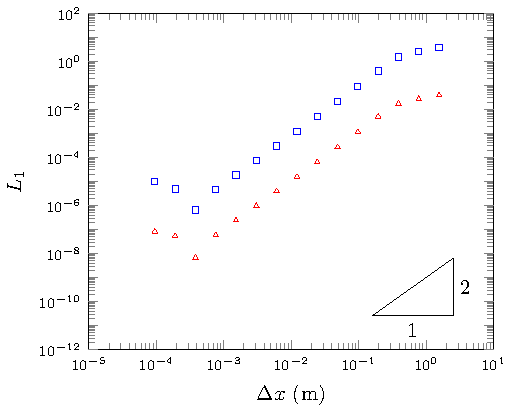
\includegraphics[width=7cm]{pics/results/soliton/L1/grim.pdf}}
\subfigure[][]{\label{fig:grimo2Enorm}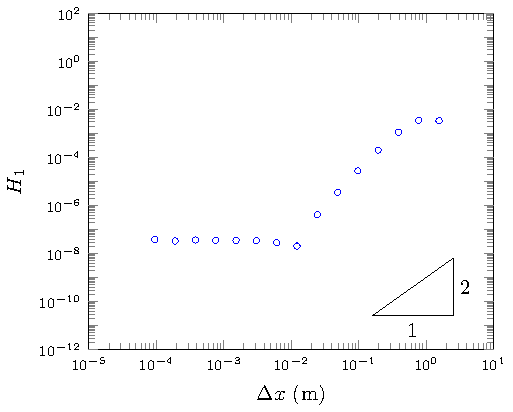
\includegraphics[width=7cm]{pics/results/soliton/H1/grim.pdf}}
\caption{On the left $L_1$ errors for $h$ ({\color{red} $\triangle$}) and $u$ ({\color{blue} $\square$}) and on the right $H_1$ ({\color{blue} $\circ$}) for the soliton problem with (a) and (b) for $\mathcal{G}$ and (c) and (d) for $\mathcal{E}$ .}
\label{fig:FDMsolnorm}
\end{figure}

\begin{figure}
\centering
\subfigure[][]{\label{fig:FDo2normC1}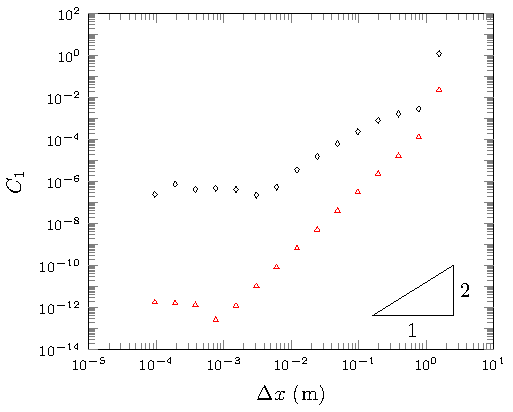
\includegraphics[width=7cm]{pics/results/soliton/C1/FDc.pdf}}
\subfigure[][]{\label{fig:grimo2normC1}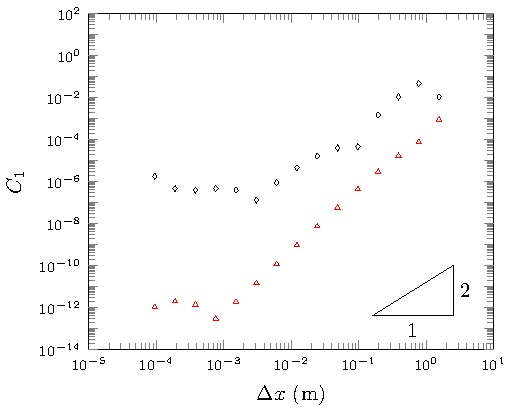
\includegraphics[width=7cm]{pics/results/soliton/C1/grim.pdf}}
\caption{$C_1$ for $h$ ({\color{red} $\triangle$}) and $uh$ ({\color{black} $\diamond$}) for numerical solutions $\mathcal{G}$ (a) and $\mathcal{E}$ (b) of the soliton problem.}
\label{fig:FDMsolnormC1}
\end{figure}
%
From Figure \ref{fig:FDMsolnorm} it can be seen that both FD methods are convergent under $L_1$ with second-order accuracy. There is however suboptimal rates of convergence for very small $\Delta x$ due to round off effects and large $\Delta x$ due to the initial conditions not being accurately represented.

From Figures \ref{fig:FDo2Enorm} and \ref{fig:grimo2Enorm} it can be seen that the FD methods conserve the Hamiltonian well and converge to the correct value of $0$ for $H_1$. Unfortunately, the point at which round off errors dominate is much earlier than for $L_1$ because $H_1$ requires more calculations than $L_1$ introducing more round off errors, although we do attain similar orders of magnitude for $L_1$ and $H_1$ before round off errors dominate. 

Lastly Figure \ref{fig:FDMsolnormC1} demonstrates conservation of both mass and momentum to at least second-order for both FD schemes. Both schemes conserve mass very well with round off error dominance occurring at the same place as for $L_1$. Momentum has the appropriate order of accuracy for larger $\Delta x$ but then stagnates as $\Delta x$ decreases. This is due to the use of a finite difference method which is not necessarily conservative for \eqref{eq:Serre_momentum} which is not in conservation law form leading to poor conservation of the momentum variable as compared to mass. Figure \ref{fig:FDMsolnormC1} however still demonstrates that these schemes are still relatively conservative and certainly there is not some drastic change in the momentum and mass in a system using these methods. 

All of these measures demonstrate that $\mathcal{G}$ and $\mathcal{E}$ are appropriate to solve highly non-linear problems with smooth initial conditions for the Serre equations. 

%--------------------------------------------------------------------------------
\section{Smoothed Dam-Break}
\label{section:smootheddambreak}
%--------------------------------------------------------------------------------
The discontinuous dam-break problem can be approximated smoothly using the hyperbolic tangent function. Such an approximation will be called a smoothed dam-break problem and will be defined as such
\begin{linenomath*}
\begin{subequations}
\begin{gather}
h(x,0) = h_0 + \frac{h_1 - h_0}{2}\left(1 + \tanh\left(\alpha\left(x_0 - x\right)\right)\right),
\end{gather}
\begin{gather}
u(x,0) = 0.0m/s.
\end{gather}
\end{subequations}
\label{eq:sdbi}
\end{linenomath*}
Where $\alpha$ is given and controls the width of the transition between the two dam-break heights of $h_0$ and $h_1$. The transition width is measured by taking the width of the smoothed dam-break problem inside which $90 \%$ of the transition between the two heights occurs which will be referred to as $\beta$. $\beta$ has the following formula independent of $h_0$, $h_1$ and $x_0$
\begin{linenomath*}
\begin{gather}
\beta = \frac{2 \tanh^{-1}\left(0.9\right)}{\alpha}.
\end{gather}
\label{eq:sdbtrans}
\end{linenomath*}
The dam break problem  of the Serre equations results in the creation of an undular bore that is very similar to the analytic solution of the dam break problem for the SWWE with oscillations occurring on top \cite{Hank-etal-2010-2034}. Undular bores for the one dimensional Serre equations were analysed by \citeN{El-etal-2006} and an expression for the lead soliton amplitude of a bore was given
\begin{linenomath*}
\begin{gather}
\frac{\Delta}{\left(a^+ + 1\right)^{1/4}} - \left(\frac{3}{4 -  \sqrt{a^+ + 1}}\right)^{21/10} \left(\frac{2}{1 + \sqrt{a^+ + 1}}\right)^{2/5} = 0
\label{eq:aplusdef}
\end{gather}
\end{linenomath*}
where $\Delta = h_2 / h_0$, $a^+$ is the leading soliton amplitude and $h_2$ is the amplitude of the bore. This measure will be used to verify that our results are sensible although $a^+$ is an estimate and not an analytic result. [] 

In the first series of experiments $h_0 = 1.0m$, $h_1 = 1.8m$ on $x \in [0m,1000m]$ for $t \in [0s,30s]$ with $x_0 = 500m$. This scenario replicates one presented by \citeN{El-etal-2006} and \citeN{Hank-etal-2010-2034} and as such serves as a comparison for the results of both with $\mathcal{E}$ and $\mathcal{G}$ and the $3$ different order FDVMs described in []. The simulations were run with various values of $\Delta x$ and $\beta$. To ensure stability especially of both FD methods a very restrictive relation of $\Delta t = 0.01 \Delta x$ was chosen. For $\mathcal{V}_2$ $\theta = 1.2$. From this description the Hamiltonian at the initial time is
\begin{gather}
\label{eqn:HamilDBinit}
\mathcal{H} (0) = 10398.6 - 0.7848\times\left[\frac{2}{\alpha} \tanh\left(500 \alpha\right)\right],
\end{gather}
which will be used to verify the produced numerical results. Applying \eqref{eq:aplusdef} with the analytic results of [] for the SWWE gives $\Delta = 1.36898$ for the bore and thus $a^+ = 1.73640$ (5 decimal places).
\begin{figure}
\centering
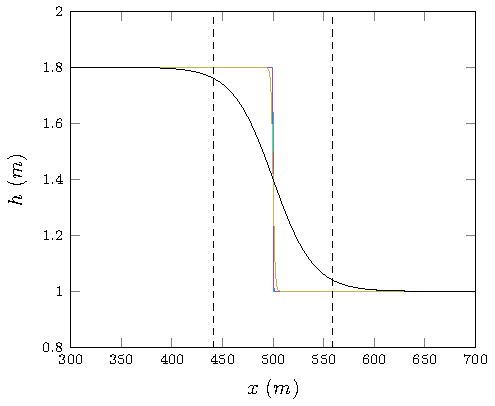
\includegraphics[width=7cm]{pics/results/SDB/init/h-figure0.pdf}
\caption{Initial conditions for the smooth dambreak problem with $\beta = 0.294$ ({\color{cyan!70!white} \solidrule}), $\beta = 1.17778$ ({\color{violet!70!white} \solidrule}), $\beta = 5.8888$ ({\color{yellow!70!black} \solidrule}) and  $\beta =117.778$ ({\color{black} \solidrule}) with reference $\beta$ interval({\color{black} \dashedrule}).}
\label{fig:dbsmoothinit}
\end{figure}

Figure \ref{fig:dbsmoothinit} shows the initial water profiles of smooth dam break problems with various $\beta$ values and indicates the interval in which $90\%$ of transition occurs for $\beta = 117.778$. The $\beta$ values in Figure \ref{fig:dbsmoothinit} are the examples that will be used to demonstrate the main scenarios for the smoothed dam-break problem in the following subsection. 
%--------------------------------------------------------------------------------
\subsection{Scenarios}
%--------------------------------------------------------------------------------
Decreasing $\Delta x$ allows the numerical method to better approximate the analytic solution to the equations. Thus the first investigation will be into the effect of $\Delta x$ on the solution of a smoothed dam break problem with fixed $\beta$. Because the smoothness of the initial conditions depends on both $\Delta x$ and $\beta$ one must be careful that the initial conditions are sufficiently smooth for the various $\Delta x$. This is of particular importance for $\mathcal{G}$ and $\mathcal{E}$ as they are not as robust as the FDVM in the presence of steep gradients.

The first and most important observation is that there are four types of behaviour as $\Delta x \rightarrow 0$ depending on the $\beta$ and the numerical method. The four scenarios are identified by the behaviour of the solutions when $\Delta x$ is small and they correspond to different results in the literature. For brevity the only given examples of these scenarios will the solutions of $\mathcal{V}_3$ although they also occurred for $\mathcal{V}_2$, $\mathcal{E}$ and $\mathcal{G}$.

The first behaviour which will be referred to as the non-oscillatory scenario has such smooth initial conditions that no oscillations were introduced by $t= 30s$, although given sufficient time an undular bore would develop. An example of this behaviour can be seen in Figure \ref{fig:o3a1dxlimflatexp} for $\beta = 117.778$. Because this is a very smooth problem we observe rapid convergence with all the numerical results being graphically identical. This scenario resembles very diffusive solutions of the shallow water wave equations in that it contains only a rarefaction and a shock with no dispersive waves. 

This convergence is also present in Figure \ref{fig:o3a1dxlimmeasure} with both the $L_1$ and $H_1$ measures. $L_1$ has been modified to use the solution of the smallest $\Delta x$ as an approximation to the analytic solution as none exists for this problem. For both measures the order of accuracy is the theoretical one, with round-off errors becoming dominant for small $\Delta x$. Since $L_1$ now compares numerical results round-off errors result in error stagnation rather than increase. For $H_1$ it can be seen that round-off errors are dominant earlier than in $L_1$ due to the increase in number of calculations. Both of these measures attain the same order of magnitude as this method applied to the soliton problem []. This suggests that this family of solutions is also a true solution of the Serre equations when $\beta = 117.778$ as well as other smoothness's that exhibit this behaviour. 


\begin{figure}
\centering
\subfigure[][]{\label{fig:o3a1dxlim}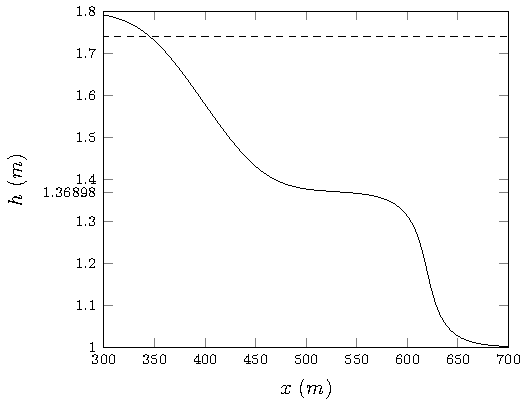
\includegraphics[width=7cm]{pics/results/SDB/numsols/alpha0.025/1-figure0.pdf}}
\caption{Numerical results of $\mathcal{V}_3$  at $t= 30s$ for the smooth dam break problem with $\beta =117.778$ for $\Delta x = 10/2^{10}$ ({\color{blue} \solidrule}), $\Delta x = 10/2^9$ ({\color{green!80!black} \solidrule}), $\Delta x = 10/2^8$ ({\color{red} \solidrule}), $\Delta x = 10/2^7$ ({\color{cyan!70!white} \solidrule}), $\Delta x = 10/2^6$ ({\color{violet!70!white} \solidrule}), $\Delta x = 10/2^5$ ({\color{yellow!70!black} \solidrule}), $\Delta x = 10/2^{4}$ ({\color{black} \solidrule}) with reference value $a^+$ ({\color{black} \dashedrule}).}
\label{fig:o3a1dxlimflatexp}
\end{figure}
%
\begin{figure}
\centering
\subfigure[][]{\label{fig:o3a1dxlimL1}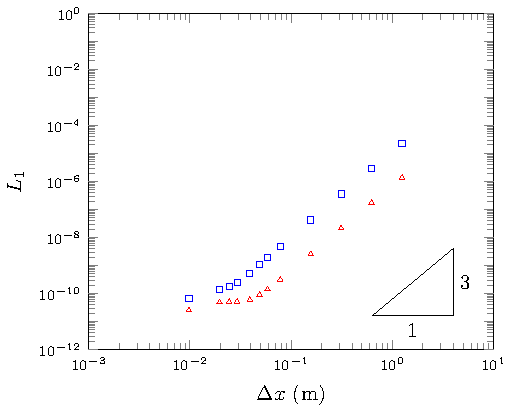
\includegraphics[width=7cm]{pics/results/SDB/Lcon/alpha0.025/1.pdf}}
\subfigure[][]{\label{fig:o3a1dxlimH}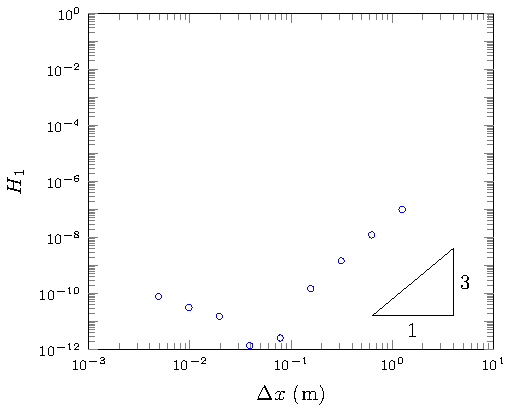
\includegraphics[width=7cm]{pics/results/SDB/Hcon/alpha0.025/1.pdf}}
\caption{$L_1$ for $h$ ({\color{red} $\triangle$}) and $u$ ({\color{blue} $\square$}) and $H_1$ ({\color{blue} $\circ$}) for $\mathcal{V}_3$'s solution for the smooth dambreak problem with $\beta =117.778$.}
\label{fig:o3a1dxlimmeasure}
\end{figure}

The second scenario will be referred to as the flat scenario due to the presence of a constant height state between the oscillations at the shock and rarefaction fan. An example of the numerical results for this scenario can be seen in Figure \ref{fig:o3a6dxlimflatexp} when $\beta = 5.8889$. This scenario corresponds to the results presented by \citeN{Hank-etal-2010-2034} and \citeN{Mitsotakis-etal-2014}. 

As $\Delta x$ decreases the solutions converge which is sensible since for the $\Delta x$ in Figure \ref{fig:o3a6dxlimflatexp} the initial conditions are smooth as can be seen in Figure \ref{fig:dbsmoothinit} and these methods have been verified for smooth problems. So that by $\Delta x = 10 / 2^8$ the solutions for higher $\Delta x$ are visually identical. There is also good agreement between the amplitude of the leading soliton and $a^+$ as well as the height of the shock wave on the plateau and the analytic value $1.36898 m$ for the SWWE. Although as $\Delta x$ is decreased the plateau seems to be slightly above this value. Since this method is well validated for smooth problems and a small $\Delta x$ has been chosen this suggests that the shock wave from a dam break problem may differ slightly for the Serre and SWWE although they are still quite close. These results also compare well to the same results in \citeN{Mitsotakis-etal-2014} with different shock speeds due to nondimensionalisation. 

The measures $L_1$ and $H_1$ also demonstrate good convergence with the expected order of accuracy in the middle of the plot. Suboptimal convergence is expected for large $\Delta x$ as the problem is not sufficiently resolved to model the oscillations and so both $H_1$ and $L_1$ suffer. For small $\Delta x$ $H_1$ becomes suboptimal due to round-off errors attaining a similar minimum to the results of $\mathcal{G}$ and $\mathcal{E}$, however this effect is masked by $L_1$ because the smallest $\Delta x$ numerical solution is the base of the comparison instead of an analytic result.

\begin{figure}
\centering
\subfigure[][]{\label{fig:o3a6dxlimz1}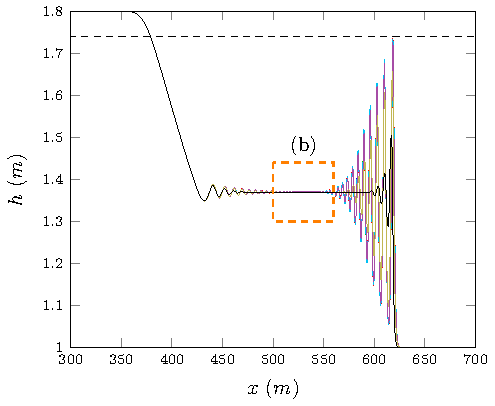
\includegraphics[width=7cm]{pics/results/SDB/numsols/alpha0.5/1-figure0.pdf}}
\subfigure[][]{\label{fig:o3a6dxlimz2}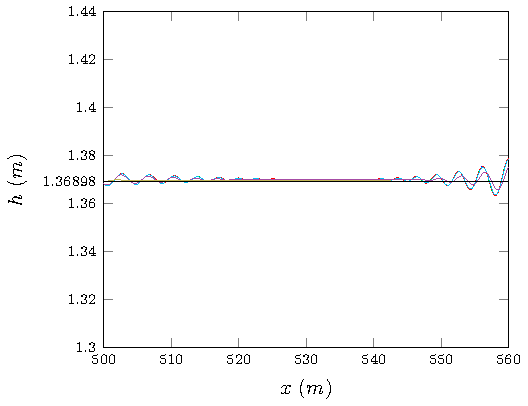
\includegraphics[width=7cm]{pics/results/SDB/numsols/alpha0.5/2-figure0.pdf}}
\caption{Numerical results of $\mathcal{V}_3$  at $t= 30s$ for the smooth dam break problem with $\beta = 5.8888$ for $\Delta x = 10/2^{10}$ ({\color{blue} \solidrule}), $\Delta x = 10/2^9$ ({\color{green!80!black} \solidrule}), $\Delta x = 10/2^8$ ({\color{red} \solidrule}), $\Delta x = 10/2^7$ ({\color{cyan!70!white} \solidrule}), $\Delta x = 10/2^6$ ({\color{violet!70!white} \solidrule}), $\Delta x = 10/2^5$ ({\color{yellow!70!black} \solidrule}), $\Delta x = 10/2^{4}$ ({\color{black} \solidrule}) with reference value $a^+$ ({\color{black} \dashedrule}).}
\label{fig:o3a6dxlimflatexp}
\end{figure}

\begin{figure}
\centering
\subfigure[][]{\label{fig:o3a2dxlimL1}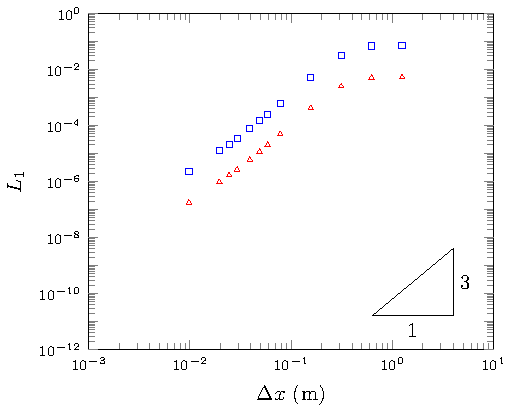
\includegraphics[width=7cm]{pics/results/SDB/Lcon/alpha0.5/1.pdf}}
\subfigure[][]{\label{fig:o3a2dxlimH}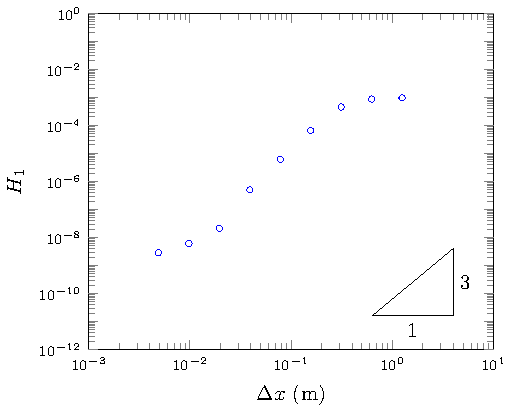
\includegraphics[width=7cm]{pics/results/SDB/Hcon/alpha0.5/1.pdf}}
\caption{$L_1$ for $h$ ({\color{red} $\triangle$}) and $u$ ({\color{blue} $\square$}) and $H_1$ ({\color{blue} $\circ$}) for $\mathcal{V}_3$'s solution for the smooth dambreak problem with $\beta = 5.8888$.}
\label{fig:o3a2dxlimmeasure}
\end{figure}

The third scenario will be referred to as the contact discontinuity scenario as in \citeN{El-etal-2006}. The contact discontinuity scenarios main feature is that the oscillations from the rarefaction fan and the shock decay and appear to meet at a point as can be seen in Figure \ref{fig:o3a9dxlimcdexp} when $\beta = 1.1778$. For the experiments performed this doesn't appear to be an stationary point but rather that the oscillations decay so quickly around the `contact discontinuity' that it appears to be the case. All the higher order methods so far have not shown a converged solution as $\Delta x$ decreases. However it does appear that convergence is likely with the solutions getting closer together, especially since for the smaller $\Delta x$ this problem is still smooth. These results also compare very well in terms of the lead soliton amplitude and the bore height reference values given on the plots. This scenario was observed by \citeN{El-etal-2006} for $\mathcal{E}$ and indeed we have replicated them for all the high order methods in this paper.

The assertion that these results are close to converged is supported by Figure \ref{fig:o3a3dxlimmeasure} for the $L^*_1$ and $H_1$ measured. As can be seen in Figure \ref{fig:o3a9dxlimz2} the final solutions have not yet even graphically converged, thus we modify $L_1$ to omit this section from $[520m,540m]$ and call this modified measure $L^*_1$. Thus $L^*_1$ demonstrates that even though this middle section has not been fully resolved we do see that there is convergence at the appropriate order outside this region. Suggesting that the effect of better resolving this contact discontinuity will only be felt locally around it and not significantly change the solution outside this region. 

$H_1$ demonstrates the appropriate order of accuracy in the Hamiltonian demonstrating that we are indeed approaching a solution to this problem as $\Delta x$ is increased, although the smallest $\Delta x$ seems to have been exceptionally fortunate and decreased by more than should be expected which should be attributed to luck than to anything more substantial. 

\begin{figure}
\centering
\subfigure[][]{\label{fig:o3a9dxlim}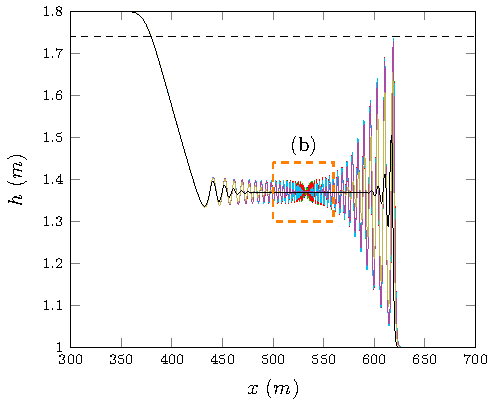
\includegraphics[width=7cm]{pics/results/SDB/numsols/alpha2.5/1-figure0.pdf}}
\subfigure[][]{\label{fig:o3a9dxlimz1}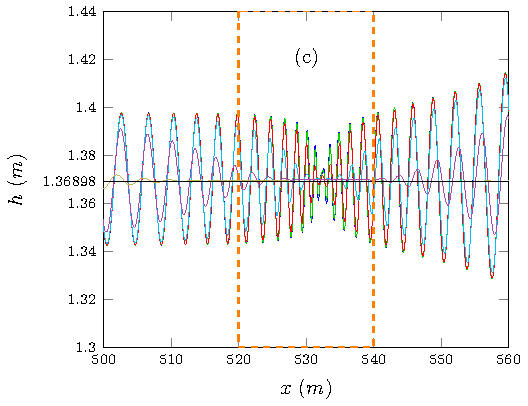
\includegraphics[width=7cm]{pics/results/SDB/numsols/alpha2.5/2-figure0.pdf}}
\subfigure[][]{\label{fig:o3a9dxlimz2}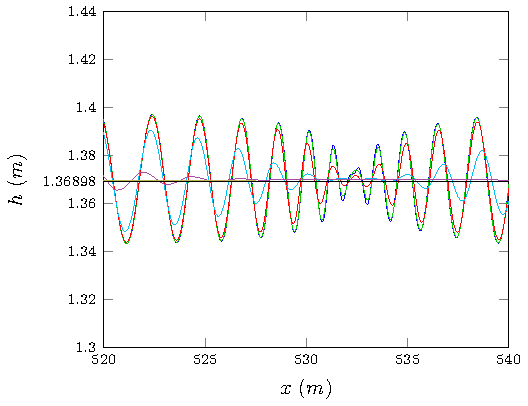
\includegraphics[width=7cm]{pics/results/SDB/numsols/alpha2.5/3-figure0.pdf}}
\caption{Numerical results of $\mathcal{V}_3$  at $t= 30s$ for the smooth dam break problem with $\beta = 1.17778$ for $\Delta x = 10/2^{10}$ ({\color{blue} \solidrule}), $\Delta x = 10/2^9$ ({\color{green!80!black} \solidrule}), $\Delta x = 10/2^8$ ({\color{red} \solidrule}), $\Delta x = 10/2^7$ ({\color{cyan!70!white} \solidrule}), $\Delta x = 10/2^6$ ({\color{violet!70!white} \solidrule}), $\Delta x = 10/2^5$ ({\color{yellow!70!black} \solidrule}), $\Delta x = 10/2^{4}$ ({\color{black} \solidrule}) with reference value $a^+$ ({\color{black} \dashedrule}).}
\label{fig:o3a9dxlimcdexp}
\end{figure}


\begin{figure}
\centering
\subfigure[][]{\label{fig:o3a3dxlimL1}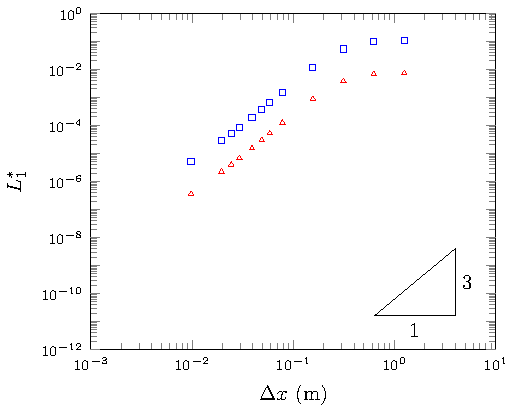
\includegraphics[width=7cm]{pics/results/SDB/Lcon/alpha2.5/1.pdf}}
\subfigure[][]{\label{fig:o3a3dxlimH}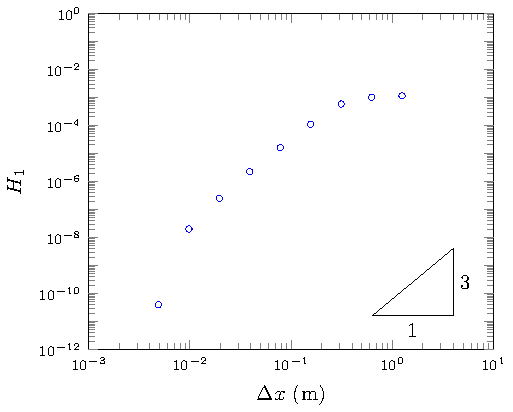
\includegraphics[width=7cm]{pics/results/SDB/Hcon/alpha2.5/1.pdf}}
\caption{$L^*_1$ for $h$ ({\color{red} $\triangle$}) and $u$ ({\color{blue} $\square$}) and $H_1$ ({\color{blue} $\circ$}) for $\mathcal{V}_3$'s solution for the smooth dambreak problem with $\beta = 1.17778$.}
\label{fig:o3a3dxlimmeasure}
\end{figure}


The fourth scenario will be referred to as the bump scenario due to the oscillations no longer decaying down towards a point but rather growing around the contact discontinuity forming a bump as can be seen in Figure \ref{fig:o3a20dxlimcdexp} for $\beta = 0.294$. This behaviour has hitherto not been published and is certainly not an expected result. 

This scenario is far from convergence in $\Delta x$, particularly in the same region as the previous scenario as can be seen in Figure \ref{fig:o3a20dxlimz2}. There are still positive signs in relation to the lead soliton amplitude and the bore height. There is also Figure \ref{fig:o3a4dxlimmeasure} which demonstrates that again outside the bump region we have the appropriate convergence and our Hamiltonian also converges. However $H_1$ is now below the order of accuracy of the scheme throughout most of the $\Delta x$'s although is appears to reach the appropriate order of accuracy at the smallest $\Delta x$. This indicates that to properly resolve these even smoothed dam break problems with similar steepness requires very small grids or higher-order schemes. Because, convergence is not assured in this scenario there is still the possibility that the wave amplitudes could explode around this point. This scenario has been observed down to $\beta = 0.00294$ with $\Delta x = 10.0/ 2^10m = 0.009765625m$, when the problem is basically a discontinuous dam-break where the amplitude of the bump is larger, but still has not exploded.

\begin{figure}
\centering
\subfigure[][]{\label{fig:o3a20dxlim}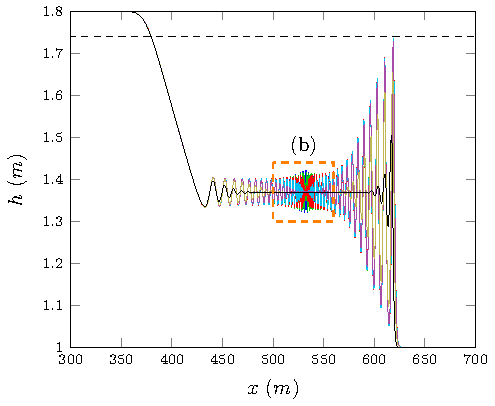
\includegraphics[width=7cm]{pics/results/SDB/numsols/alpha10/1-figure0.pdf}}
\subfigure[][]{\label{fig:o3a20dxlimz1}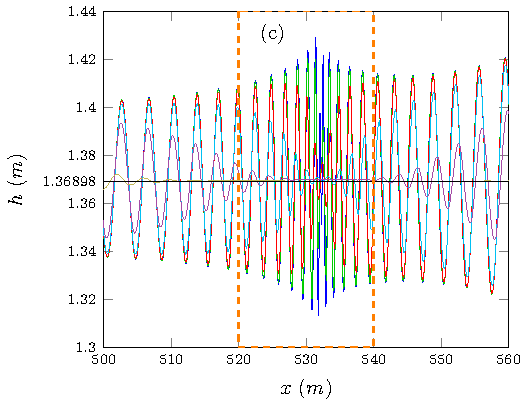
\includegraphics[width=7cm]{pics/results/SDB/numsols/alpha10/2-figure0.pdf}}
\subfigure[][]{\label{fig:o3a20dxlimz2}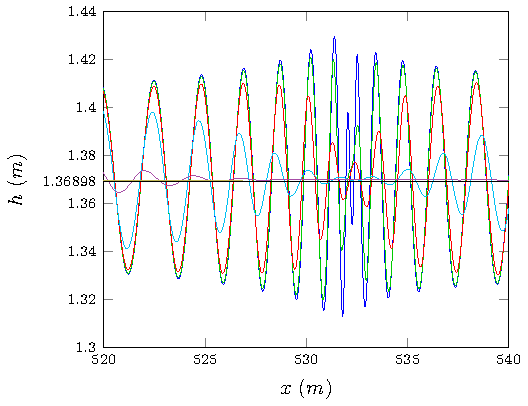
\includegraphics[width=7cm]{pics/results/SDB/numsols/alpha10/3-figure0.pdf}}
\caption{Numerical results of $\mathcal{V}_3$  at $t= 30s$ for the smooth dam break problem with $\beta = 0.294$ for $\Delta x = 10/2^{10}$ ({\color{blue} \solidrule}), $\Delta x = 10/2^9$ ({\color{green!80!black} \solidrule}), $\Delta x = 10/2^8$ ({\color{red} \solidrule}), $\Delta x = 10/2^7$ ({\color{cyan!70!white} \solidrule}), $\Delta x = 10/2^6$ ({\color{violet!70!white} \solidrule}), $\Delta x = 10/2^5$ ({\color{yellow!70!black} \solidrule}), $\Delta x = 10/2^{4}$ ({\color{black} \solidrule}) with reference value $a^+$ ({\color{black} \dashedrule}).}
\label{fig:o3a20dxlimcdexp}
\end{figure}

\begin{figure}
\centering
\subfigure[][]{\label{fig:o3a4dxlimL1}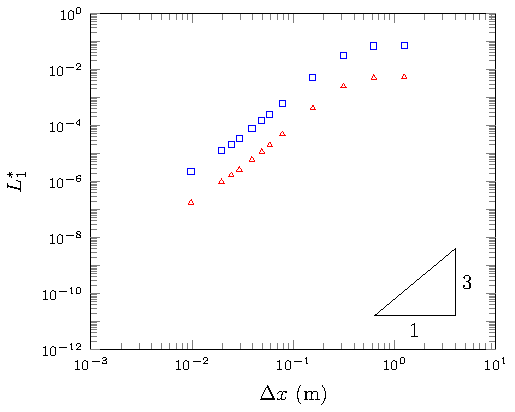
\includegraphics[width=7cm]{pics/results/SDB/Lcon/alpha10/1.pdf}}
\subfigure[][]{\label{fig:o3a4dxlimH}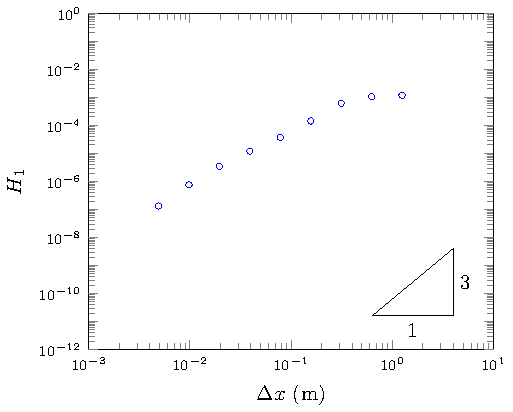
\includegraphics[width=7cm]{pics/results/SDB/Hcon/alpha10/1.pdf}}
\caption{$L^*_1$ for $h$ ({\color{red} $\triangle$}) and $u$ ({\color{blue} $\square$}) and $H_1$ ({\color{blue} $\circ$}) for $\mathcal{V}_3$'s solution for the smooth dambreak problem with $\beta = 0.294$.}
\label{fig:o3a4dxlimmeasure}
\end{figure}

Since this result is unexpected and not as supported as the contact discontinuity scenario in the literature \cite{El-etal-2006} [USSR paper about plasmas]. The first check should be very different numerical methods such as $\mathcal{G}$ and $\mathcal{E}$ to test if some numerical effect from the reformulation of the Serre equations or the elliptic solver are the cause. For comparison all methods discussed in this paper with the same parameters as the example above are plotted in Figure \ref{fig:MODlim}. The first observation of this figure is that $\mathcal{V}_1$ has not recovered this behaviour. This is because as noted in [], $\mathcal{V}_1$ is very diffusive which the behaviour seems to be very sensitive to. To resolve such behaviour for $\mathcal{V}_1$ would require incredibly small $\Delta x$ and as such we have not seen this behaviour yet, although the other methods together demonstrate that we would eventually see it. The next is that all high order methods recover this bump behaviour and disagree only in the region around the contact discontinuity. The main difference in the oscillations is their phase and amplitude with the dispersive FD methods resulting in larger waves than the diffusive FDVM. Dispersive methods decrease oscillation amplitude and number as $\Delta x$ is decreased as can be seen in Figure \ref{fig:FDa6lim}. Thus since the FDVM are diffusive and therefore do the opposite the true analytic solution should then exist between these two results, which would still be a bump around the contact discontinuity. Finally it can be seen that $\mathcal{V}_2$, $\mathcal{V}_3$ and $\mathcal{E}$ are very similar. [because they are very similar, or because we are closed to converged]

However, using the more robust and conservative $\mathcal{V}_i$ schemes results in $\mathcal{H}(30s) < \mathcal{H}(0s)$ so energy is only lost where as $\mathcal{G}$ and $\mathcal{E}$ can both gain energy as can be seen in Figure \ref{fig:o3a4dxHallsign}. This is desirable because [].???
\begin{figure}
\centering
\subfigure[][]{\label{fig:o3a4dxH1propFDVM}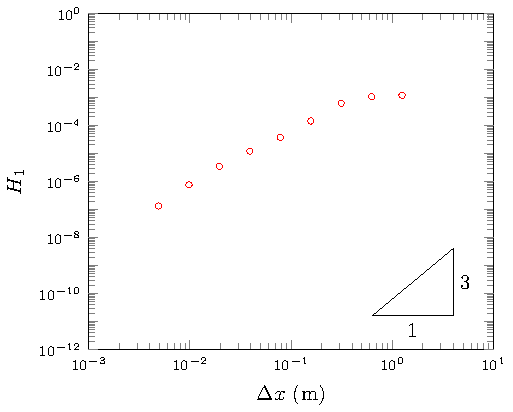
\includegraphics[width=7cm]{pics/results/SDB/Hcon/alpha10signs/o3.pdf}}
\subfigure[][]{\label{fig:o3a4dxH1propFD}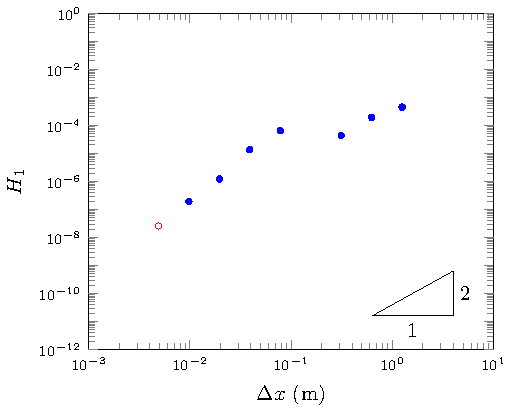
\includegraphics[width=7cm]{pics/results/SDB/Hcon/alpha10signs/FDc.pdf}}
\caption{$H_1$ for $\mathcal{V}_3$ (a) and $\mathcal{G}$'s (b) solution for the smooth dambreak problem at $t = 30s$ with $\beta = 0.294$ demonstrating when $\mathcal{H}(0s) \ge \mathcal{H}(30s)$ ({\color{red} $\circ$}) and $\mathcal{H}(0s) < \mathcal{H}(30s)$ ({\color{blue} $\bullet$}).}
\label{fig:o3a4dxHallsign}
\end{figure}


\begin{figure}
\centering
\subfigure[][]{\label{fig:MODh}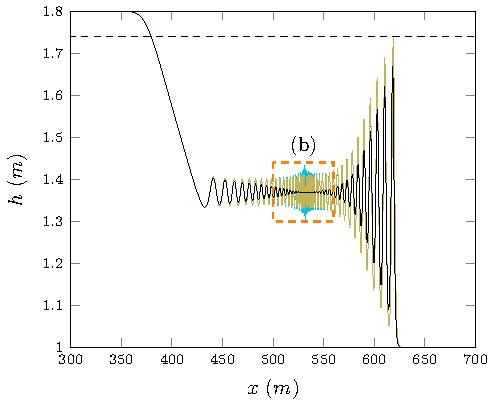
\includegraphics[width=7cm]{pics/results/SDB/numsols/modelcomppalpha10dx10/1-figure0.pdf}}
\subfigure[][]{\label{fig:MODh1}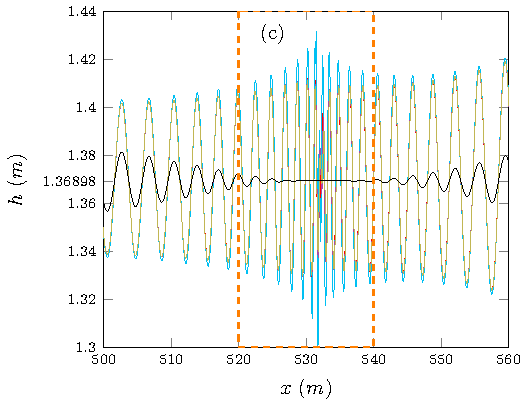
\includegraphics[width=7cm]{pics/results/SDB/numsols/modelcomppalpha10dx10/2-figure0.pdf}}
\subfigure[][]{\label{fig:MODh2}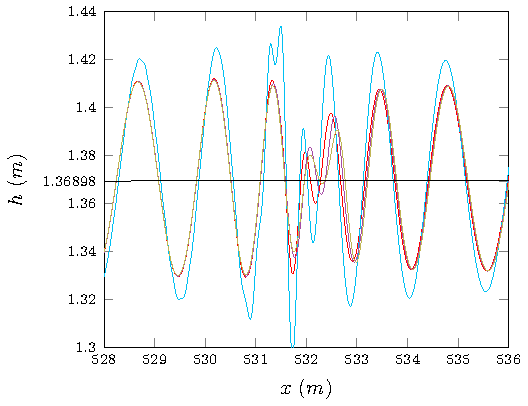
\includegraphics[width=7cm]{pics/results/SDB/numsols/modelcomppalpha10dx10/4-figure0.pdf}}
\caption{Numerical results for the smooth dam break problem with $\beta = 0.294$ and $\Delta x = 10/2^{10}$
for $\mathcal{E}$ ({\color{red} \solidrule}), $\mathcal{G}$ ({\color{cyan!70!white} \solidrule}), $\mathcal{V}_3$ ({\color{violet!70!white} \solidrule}), $\mathcal{V}_2$ ({\color{yellow!70!black} \solidrule}) and $\mathcal{V}_1$ ({\color{black} \solidrule}) with reference value $a^+$ ({\color{black} \dashedrule}).}
\label{fig:MODlim}
\end{figure}

\begin{figure}
\centering
\subfigure[][]{\label{fig:FDa6h}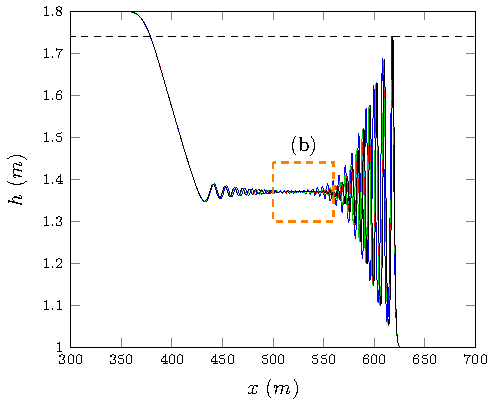
\includegraphics[width=7cm]{pics/results/SDB/numsols/FDcalpha0.5/1-figure0.pdf}}
\subfigure[][]{\label{fig:FDa6hz}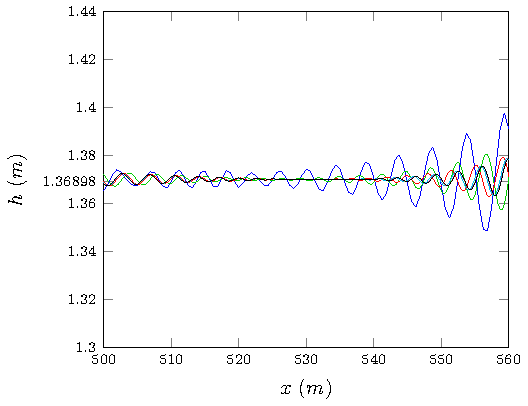
\includegraphics[width=7cm]{pics/results/SDB/numsols/FDcalpha0.5/2-figure0.pdf}}
\caption{Numerical results of $\mathcal{G}$  at $t= 30s$ for the smooth dam break problem with $\beta = 5.8888$ for $\Delta x = 10/2^{4}$ ({\color{blue} \solidrule}), $\Delta x = 10/2^5$ ({\color{green!80!black} \solidrule}), $\Delta x = 10/2^6$ ({\color{red} \solidrule}), $\Delta x = 10/2^7$ ({\color{cyan!70!white} \solidrule}), $\Delta x = 10/2^8$ ({\color{violet!70!white} \solidrule}), $\Delta x = 10/2^9$ ({\color{yellow!70!black} \solidrule}), $\Delta x = 10/2^{10}$ ({\color{black} \solidrule}) with reference value $a^+$ ({\color{black} \dashedrule}).}
\label{fig:FDa6lim}
\end{figure}


There is still the possibility that these solutions are caused by some numerical phenomena such as these methods not properly handling contact discontinuities, more research into this topic should be undertaken. However, the agreement of all the discussed methods of sufficiently high order indicates that these results are representative of actual solutions of the dam break problem for the Serre equations. Thus the following section of this paper will be concerned with some numerical investigation into this bump phenomenon. 



%--------------------------------------------------------------------------------
\subsection{Source}
%--------------------------------------------------------------------------------
The first test of these results will be of its evolution through time, thus an experiment was run with the same parameters for $t \in [0,100s]$. The results for $\beta = 0.294$ and $\Delta x = 10/2^{10}$ are presented in Figure \ref{fig:FVlonga20}. It can be seen that this bump has persisted through time although it has shrunk from roughly $0.11m$ at $t = 30s$ to $0.06m$ at $t = 100s$ in accordance with the other waves in this midsection. The waves at the front have actually increased in amplitude as time has progressed, this growth can be seen in Figure \ref{fig:FVlonga20aplus} which tracks the lead soliton amplitude against time. It can be seen that the lead soliton amplitude has passed the estimate given by \citeN{El-etal-2006}, however it still appears to be approaching an asymptotic value and the two values at $t = 100s$ differ only by $1.4\%$ which fits in with the numerical results of that paper. This suggests that as time goes on the middle section will retain a similar shape while its oscillations shrink uniformly, while the waves at the front of the shocks height will approach the asymptotic value which is close but differs from the estimate by \citeN{El-etal-2006}.

%long time 
\begin{figure}
\centering
\subfigure[][]{\label{fig:FVlonga20h}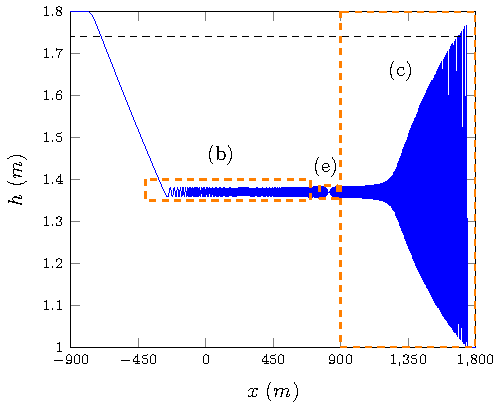
\includegraphics[width=7cm]{pics/results/SDB/numsols/300s/h0t300s.pdf}}
\subfigure[][]{\label{fig:FVlonga20hf}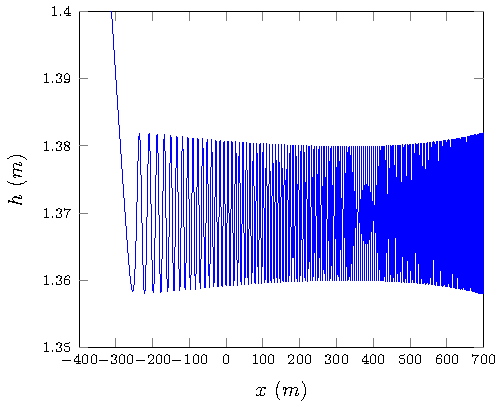
\includegraphics[width=7cm]{pics/results/SDB/numsols/300s/h2t300s.pdf}}
\subfigure[][]{\label{fig:FVlonga20hb}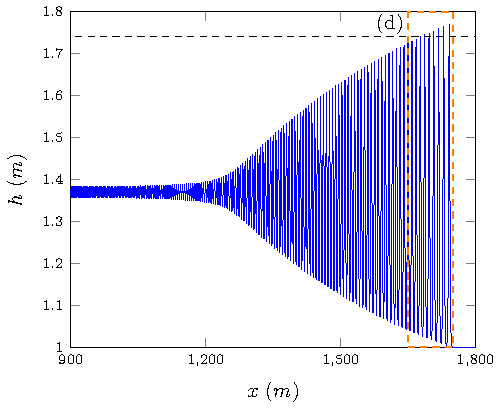
\includegraphics[width=7cm]{pics/results/SDB/numsols/300s/h1t300s.pdf}}
\subfigure[][]{\label{fig:FVlonga20hz}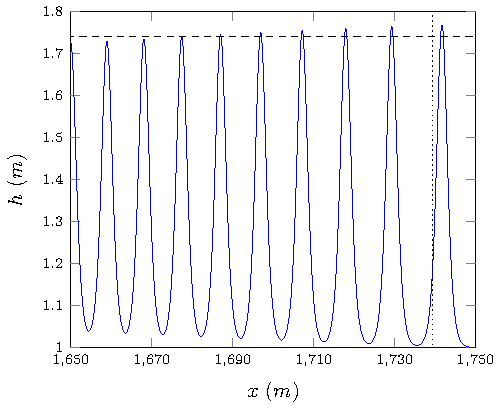
\includegraphics[width=7cm]{pics/results/SDB/numsols/300s/h4t300s.pdf}}
\subfigure[][]{\label{fig:FVlonga20hz}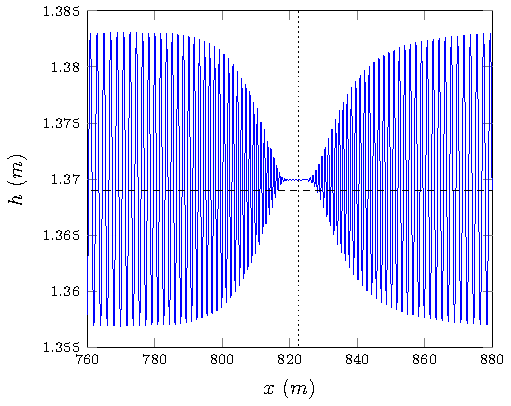
\includegraphics[width=7cm]{pics/results/SDB/numsols/300s/h3t300s.pdf}}
\caption{Smooth dam break problem at $t=300s$ for $\mathcal{V}_3$ with $\beta = 0.294$ for $\Delta x = 10/2^{9}$ ({\color{blue} \solidrule}) with reference values  $a^+$ ({\color{black} \dashedrule}) ((a), (b)), $h_2$ ({\color{black} \dashedrule})(d) and $x_2$ ({\color{black} \dotrule{0.04\textwidth}}) (d).}
\label{fig:FVlonga20}
\end{figure}

\begin{figure}
\centering
\subfigure[][]{\label{fig:FVlonga20a}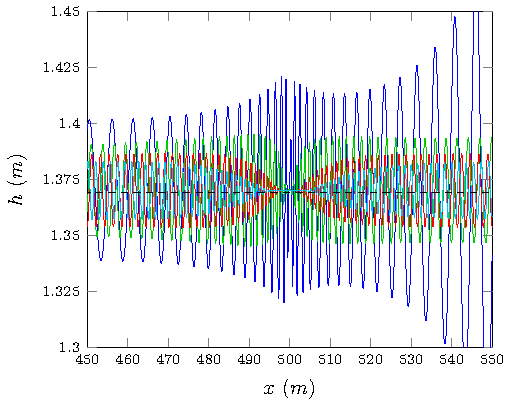
\includegraphics[width=7cm]{pics/results/SDB/numsols/300s/difftimescenteredat500m.pdf}}
\caption{Water profile shifted by $u_2 \times t$ for the numerical solution of the smoothed dam break with $\mathcal{V}_3$, $\beta = 0.294$ and $\Delta x = 10/2^{9}$ at $t=30s$ ({\color{blue} \solidrule}), $t=100s$ ({\color{green!80!black} \solidrule}), $t=200s$ ({\color{red} \solidrule}) and $t=300s$ ({\color{cyan!70!white} \solidrule}).}
\label{fig:FVlongcemt500}
\end{figure}

\begin{figure}
\centering
\subfigure[][]{\label{fig:FVlonga20a}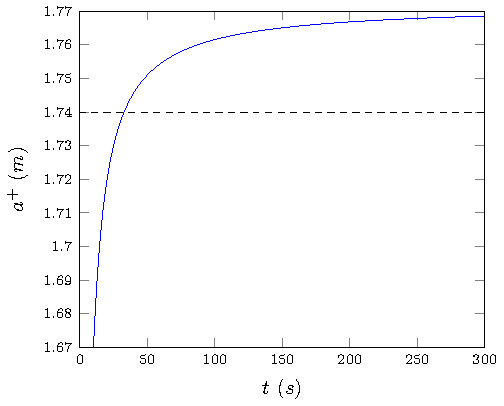
\includegraphics[width=7cm]{pics/results/SDB/numsols/300s/a.pdf}}
\caption{Lead soliton height plotted over time for the smooth dam break problem at $t=300s$ for $\mathcal{V}_3$ with $\beta = 0.294$ for $\Delta x = 10/2^{9}$ ({\color{blue} \solidrule}) with reference value $a^+$ ({\color{black} \dashedrule}).}
\label{fig:FVlonga20aplus}
\end{figure}

%coarsefinecomparison
\begin{figure}
\centering
\subfigure[][]{\label{fig:FVcomplonga20h}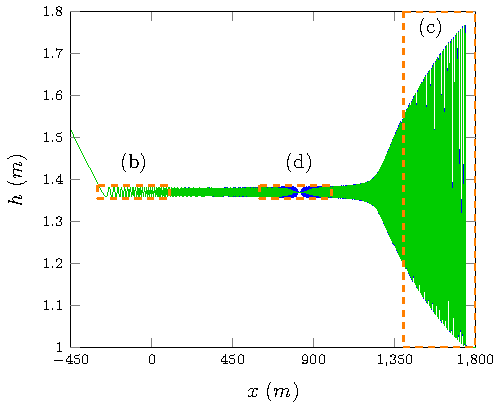
\includegraphics[width=7cm]{pics/results/SDB/numsols/300s/CF0t300.pdf}}
\subfigure[][]{\label{fig:FVcomplonga20hf}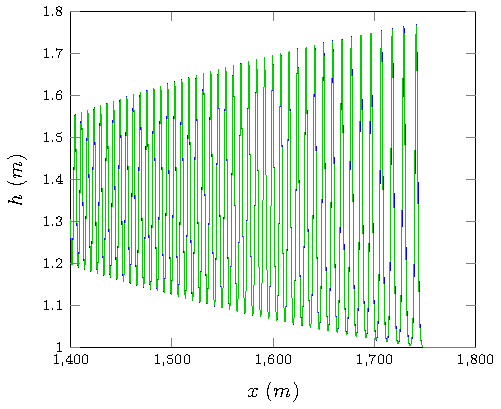
\includegraphics[width=7cm]{pics/results/SDB/numsols/300s/CF2t300.pdf}}
\subfigure[][]{\label{fig:FVcomplonga20hb}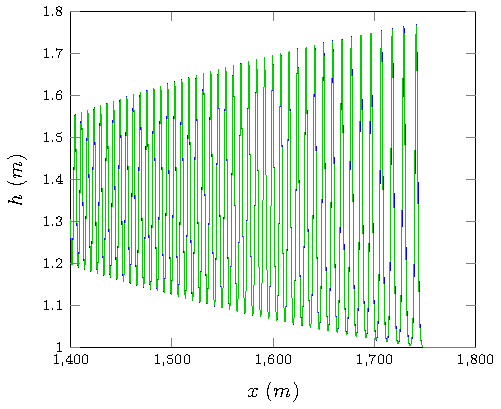
\includegraphics[width=7cm]{pics/results/SDB/numsols/300s/CF2t300.pdf}}
\subfigure[][]{\label{fig:FVcomplonga20hz}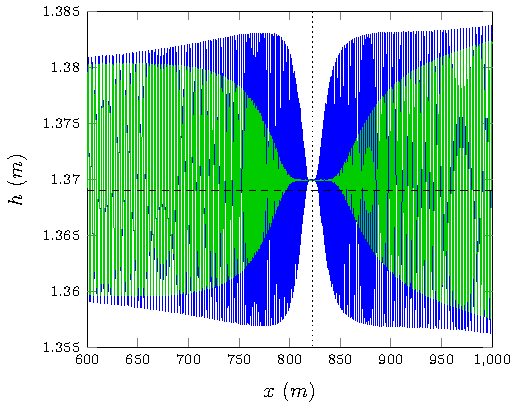
\includegraphics[width=7cm]{pics/results/SDB/numsols/300s/CF3t300.pdf}}
\caption{Smooth dam break problem at $t=300s$ for $\mathcal{V}_3$ with $\beta = 0.294$ for $\Delta x = 10/2^{9}$ ({\color{blue} \solidrule}) with reference values $h_2$ ({\color{black} \dashedrule})(d) and $x_2$ ({\color{black} \dotrule{0.04\textwidth}}) (d).}
\label{fig:FVcomplonga20}
\end{figure}


%energy break down

The Hamiltonian \eqref{eqn:Hamildef} has $3$ terms representing in order, kinetic energy , gravitational potential energy and lastly a sort of dispersive energy. It might be expected that the these rapid oscillations of the undular bore such as in Figure \ref{fig:FVlonga20} would result in significant dispersive energies. However, Figure \ref{fig:PHTa12all} demonstrates that this is not the case, with the total dispersive energy in the system being insignificant relative to the others. This plot also demonstrates that even with dispersive terms the drivers of change in the dam break problem are the transfer of gravitational potential energy into kinetic energy which occurs very slowly.

\begin{figure}
\centering
\subfigure[][]{\label{fig:PHTa12}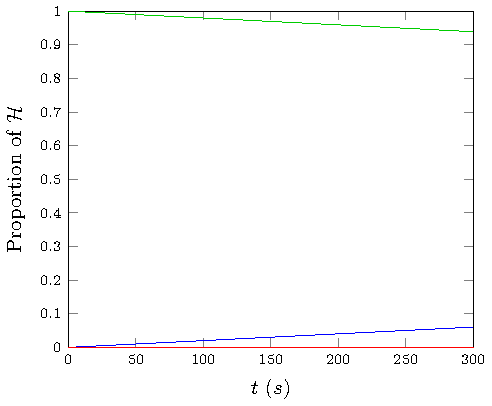
\includegraphics[width=7cm]{pics/results/SDB/numsols/300s/HFT-figure0.pdf}}
\subfigure[][]{\label{fig:PHTa12z}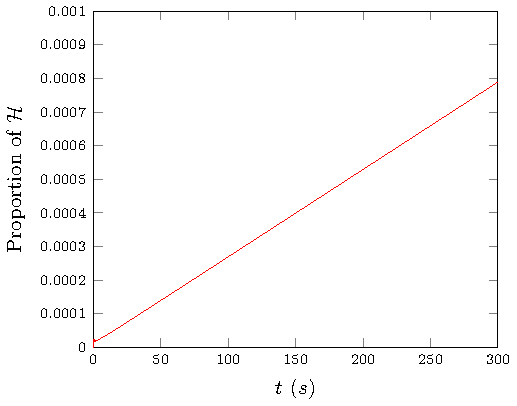
\includegraphics[width=7cm]{pics/results/SDB/numsols/300s/TT-figure0.pdf}}
\caption{Proportion of $\mathcal{H}$ made up by $\mathcal{H}_1$ ({\color{blue} \solidrule}) , $\mathcal{H}_2$ ({\color{green!80!black} \solidrule}) and $\mathcal{H}_3$ ({\color{red} \solidrule})  for $\mathcal{V}_3$ solution of the smooth dam break with $\beta = 0.2944$ and $\Delta x = 10/2^{9}$ over time.}
\label{fig:PHTa12all}
\end{figure}


%uh comparison
From [] the analytic solution for the SWWE can be obtained for the height $h_2$ and speed of the bore $u_2$, the solution of the dam break problem for the Serre equations consists of oscillations around these values [], although perhaps slightly different values as noted above[]. Thus using these analytic values a plot of both $h$ and $u$ can be superimposed, in our case by altering the $u$ value. In Figure \ref{fig:UHcompall} this has been done by adding $0.29400$ to the values of $u$. From this figure it can be seen that maxima and minima for both values line up very nicely with the distinction being that in front of the contact discontinuity the oscillations are in phase whereas behind if they are antiphase. This causes the waves peaks and thus waves to travel away from the contact discontinuity. 

\begin{figure}
\centering
\subfigure[][]{\label{fig:UHcomp1}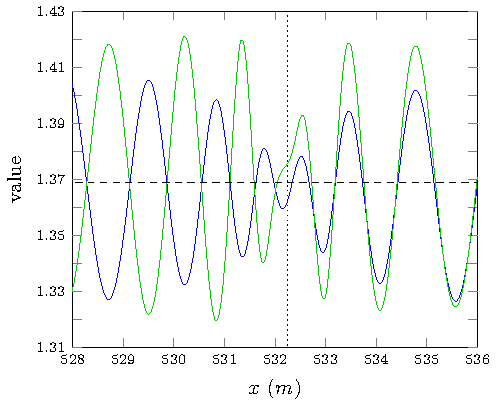
\includegraphics[width=7cm]{pics/results/SDB/numsols/300s/uh0t30.pdf}}
\subfigure[][]{\label{fig:UHcomp2}\includegraphics[width=7cm]{pics/results/SDB/numsols/300s/uh1t30.pdf}}
\subfigure[][]{\label{fig:UHcomp3}\includegraphics[width=7cm]{pics/results/SDB/numsols/300s/uh2t30.pdf}}
\subfigure[][]{\label{fig:UHcomp4}\includegraphics[width=7cm]{pics/results/SDB/numsols/300s/uh3t30.pdf}}
\caption{adjusted $u$ ({\color{blue} \solidrule}) and $h$ ({\color{green!80!black} \solidrule}) for $\mathcal{V}_3$ solution of the smooth dam break with $\beta = 0.2944$ and $\Delta x = 10/2^{9}$ at $t=30s$.}
\label{fig:UHcomp30sall}
\end{figure}

\begin{figure}
\centering
\subfigure[][]{\label{fig:UHcomp1}\includegraphics[width=7cm]{pics/results/SDB/numsols/300s/uh0t300.pdf}}
\subfigure[][]{\label{fig:UHcomp2}\includegraphics[width=7cm]{pics/results/SDB/numsols/300s/uh1t300.pdf}}
\subfigure[][]{\label{fig:UHcomp3}\includegraphics[width=7cm]{pics/results/SDB/numsols/300s/uh2t300.pdf}}
\subfigure[][]{\label{fig:UHcomp4}\includegraphics[width=7cm]{pics/results/SDB/numsols/300s/uh3t300.pdf}}
\caption{adjusted $u$ ({\color{blue} \solidrule}) and $h$ ({\color{green!80!black} \solidrule}) for $\mathcal{V}_3$ solution of the smooth dam break with $\beta = 0.2944$ and $\Delta x = 10/2^{9}$ at $t=300s$. }
\label{fig:UHcomp300sall}
\end{figure}

%cd speed
Finally it is of interest to see at what speed the contact discontinuity travels, because contact discontinuities are supposed to travel at the velocity of the bore[]. Since as stated before there are analytic solutions for these values for the SWWE, the numerical results can be compared to this. To investigate this $h_1$ was varied to allow for different aspect ratios and thus different bore speeds. The results are plotted in Figure \ref{fig:CDspeed} from which it is quite clear that this discontinuity does in fact travel at the bore speed for a range of aspect ratios. 
\begin{figure}
\centering
\subfigure[][]{\label{fig:CDspeed1}\includegraphics[width=7cm]{pics/results/SDB/CDspeed/speed.pdf}}
\caption{$v_{DB}$ ({\color{blue} \solidrule}) and $v_{CD}$ ({\color{red} $\circ$})  for $\mathcal{V}_3$ solution of the various smooth dam break problems with $\beta = 0.2944$ and $\Delta x = 10/2^{10}$ at $t=100s$.}
\label{fig:CDspeed}
\end{figure}


%--------------------------------------------------------------------------------
\section{Conclusions}
\label{section:Conclusions}
%--------------------------------------------------------------------------------

%--------------------------------------------------------------------------------
\section{Acknowledgements}
%--------------------------------------------------------------------------------

%--------------------------------------------------------------------------------
\bibliography{Serre_ASCE}
%--------------------------------------------------------------------------------

\end{document}
